\section{Conclusion}

\subsection{Summary}
[WHAT DID WE ARRIVE AT. ANSWERS TO OUR LEADING QUESTIONS]

Is it possible. Is it feasible.




\subsection{Future Work}
INTROTEXT

Because of the rapid development in the fields discussed in this report, much of what we've gone through could be improved in the future. With new \textit{Augmented Reality} and \textit{Mixed Reality} hardware being developed by big franchises, such as Facebook \cite{facebookAR}, the performance will increase ever so rapidly.

The model used also only included the pieces to one furniture, but one could easily include more in the future by gathering data for other furniture parts.

\subsubsection{Wearable}
One improvement of our application would be to port it to, not only hand-held devices, but also the headgear, thus allowing the user to building with both hands and never have to pause during the assembly process.

\subsubsection{Detecting smaller objects}
Another issue with our model is that we are unable to detect screws and bolts because of their 
comparatively small size, instead, we just inform the user that screws should be used during a particular step using animations.
This issue could possibly be fixed by adapting our model into taking account to smaller objects.
Some future work could be to investigate whether it is possible.

\subsubsection{Mask RCNN}
Since there was a lot of confusion around the green markings from the user tests, it would be an
improvement to only mark the exact position of the part and not the surrounding floor.
For this application only the bounding box of the 2D image is known, not the floor where it lays.

A possible solution to this in the future could be to implement a Mask RCNN network. However, 
the problem with this type right now is that it does not work in real time applications (definitely not on mobile devices).
If this would get better it could be implemented in the app for a much nicer user experience.

\subsubsection{Starting the app in the ARScene}
When comparing to other AR Applications in the App Store, a lot of them starts right in the AR 
scene. This seems to be somewhat of a convention in the AR community.

We chose to have the user select the furniture before entering the AR scene to make the GUI
implementation easier. However, it could be changed so that the furniture could be selected
either from an overlay or a bottom card design over the AR scene view.

\subsubsection{Shared AR experience}
Ever since ARKit 2.0 was released, it is possible to share an AR experience with another user.
Since the app already utilizes ARKit 2.0 it would be relatively simple to implement a shared 
experience. The shared experience could make it easier for multiple people to work together to
assemble a furniture. Big furnitures are rarely assembled by just one person.

\subsubsection{Voiced instructions}
Reading instructions on the screen while viewing a video preview is not the most intuitive in an
AR environment. The eyes are mostly focused on what is going on in the environment and text
instructions given on an overlay can easily be missed if they are subtle.

Furthermore, people with hard of seeing could have a hard time with both reading the instructions
and seeing the 3D models. This problem can be solved by introducing voiced instructions in the app.

\subsubsection{Finding the anchor points with object detection}
Since screws were to small to detect, so are the anchor points on the furniture parts that connect
each other.
An improvement in the future could be to try to detect the exact anchor points on the
real furniture parts and rendering the virtual object right on that location. This would
require more work on training the neural net to detect those small parts and probably
higher resolution on the images.

\subsubsection{Make it scalable}
The application only supports one furniture. For a full scale application it would need to support
many more furnitures. For a complete catalogue there could exist hundreds of furnitures.

To add support for a new furniture in the app the following steps are needed:

\begin{list}{•}
\item Take at least 50 pictures of every furniture part
\item Train a neural net to recognize those parts and import the model into Xcode
\item Add an instruction set on how to put the furniture together
\item Add 3D models of all the parts and the fully assembled model
\item Add anchor points and screw points to the models
\end{list}

The problem of making the app scalable is the size of the ML-model. For many furnitures it could
easily be the size of 1 GB or more. A way to solve this is to have an downloadable ML-model for each 
furniture. These could be fetched from a database before starting the assembly session.

All the other instructions, geometry, anchor- and screw points could also be fetched from a database.

\subsubsection{Occlusion problem in AR}
\begin{figure}[hbtp]
\begin{center}
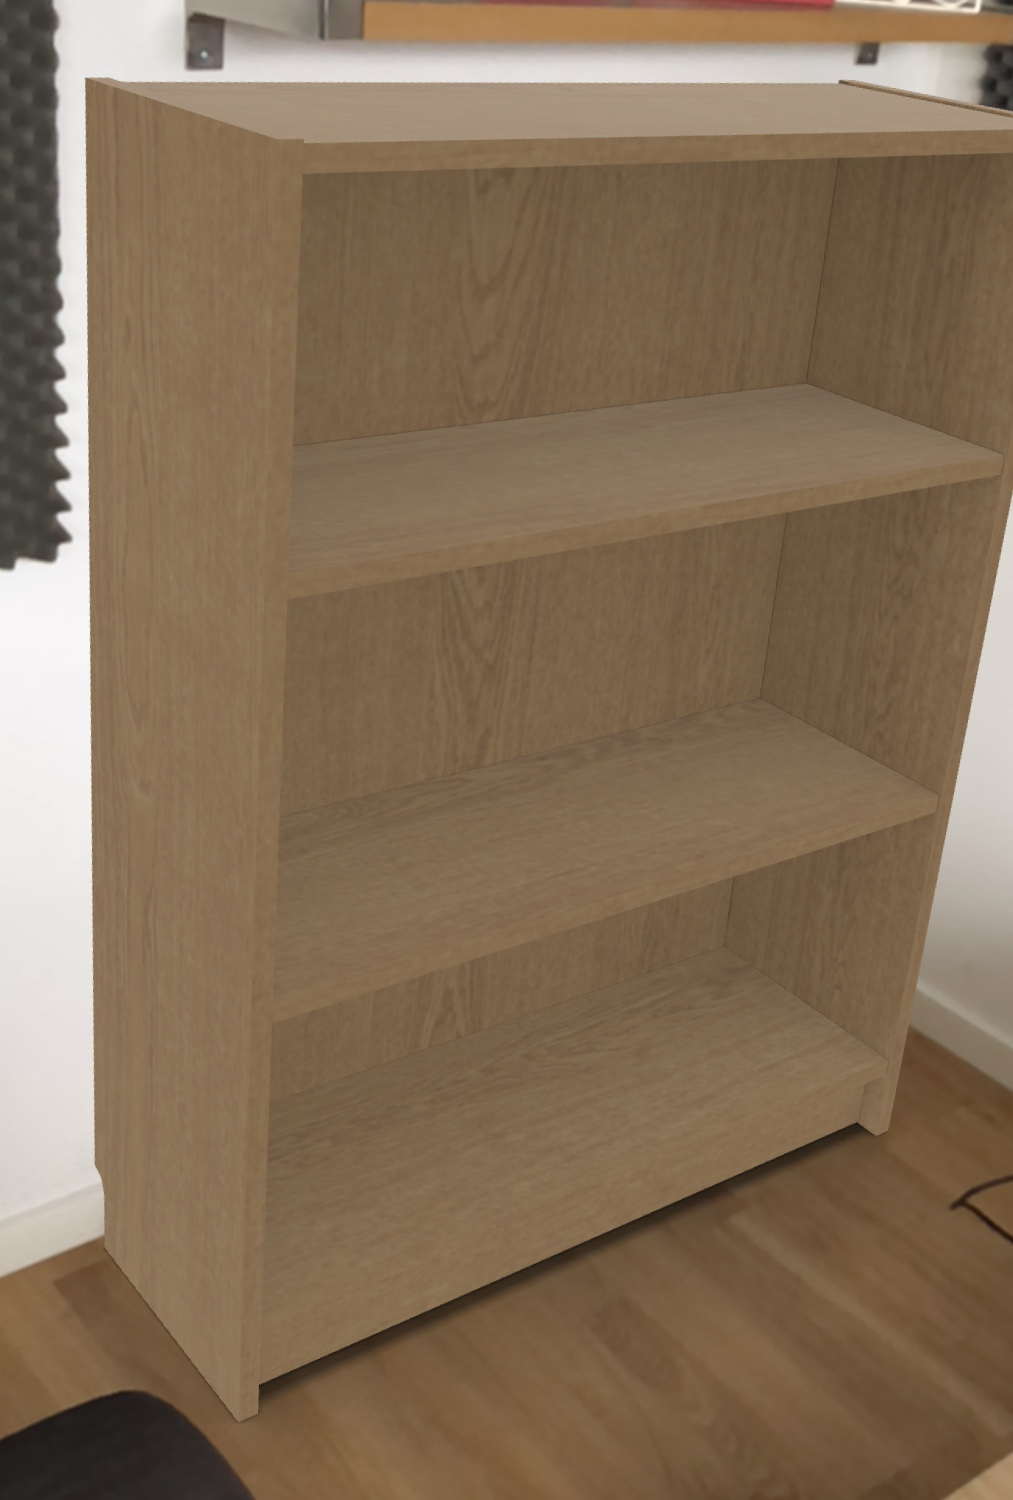
\includegraphics[width = 0.25\textwidth]{./Images/overlapping2.jpg} 
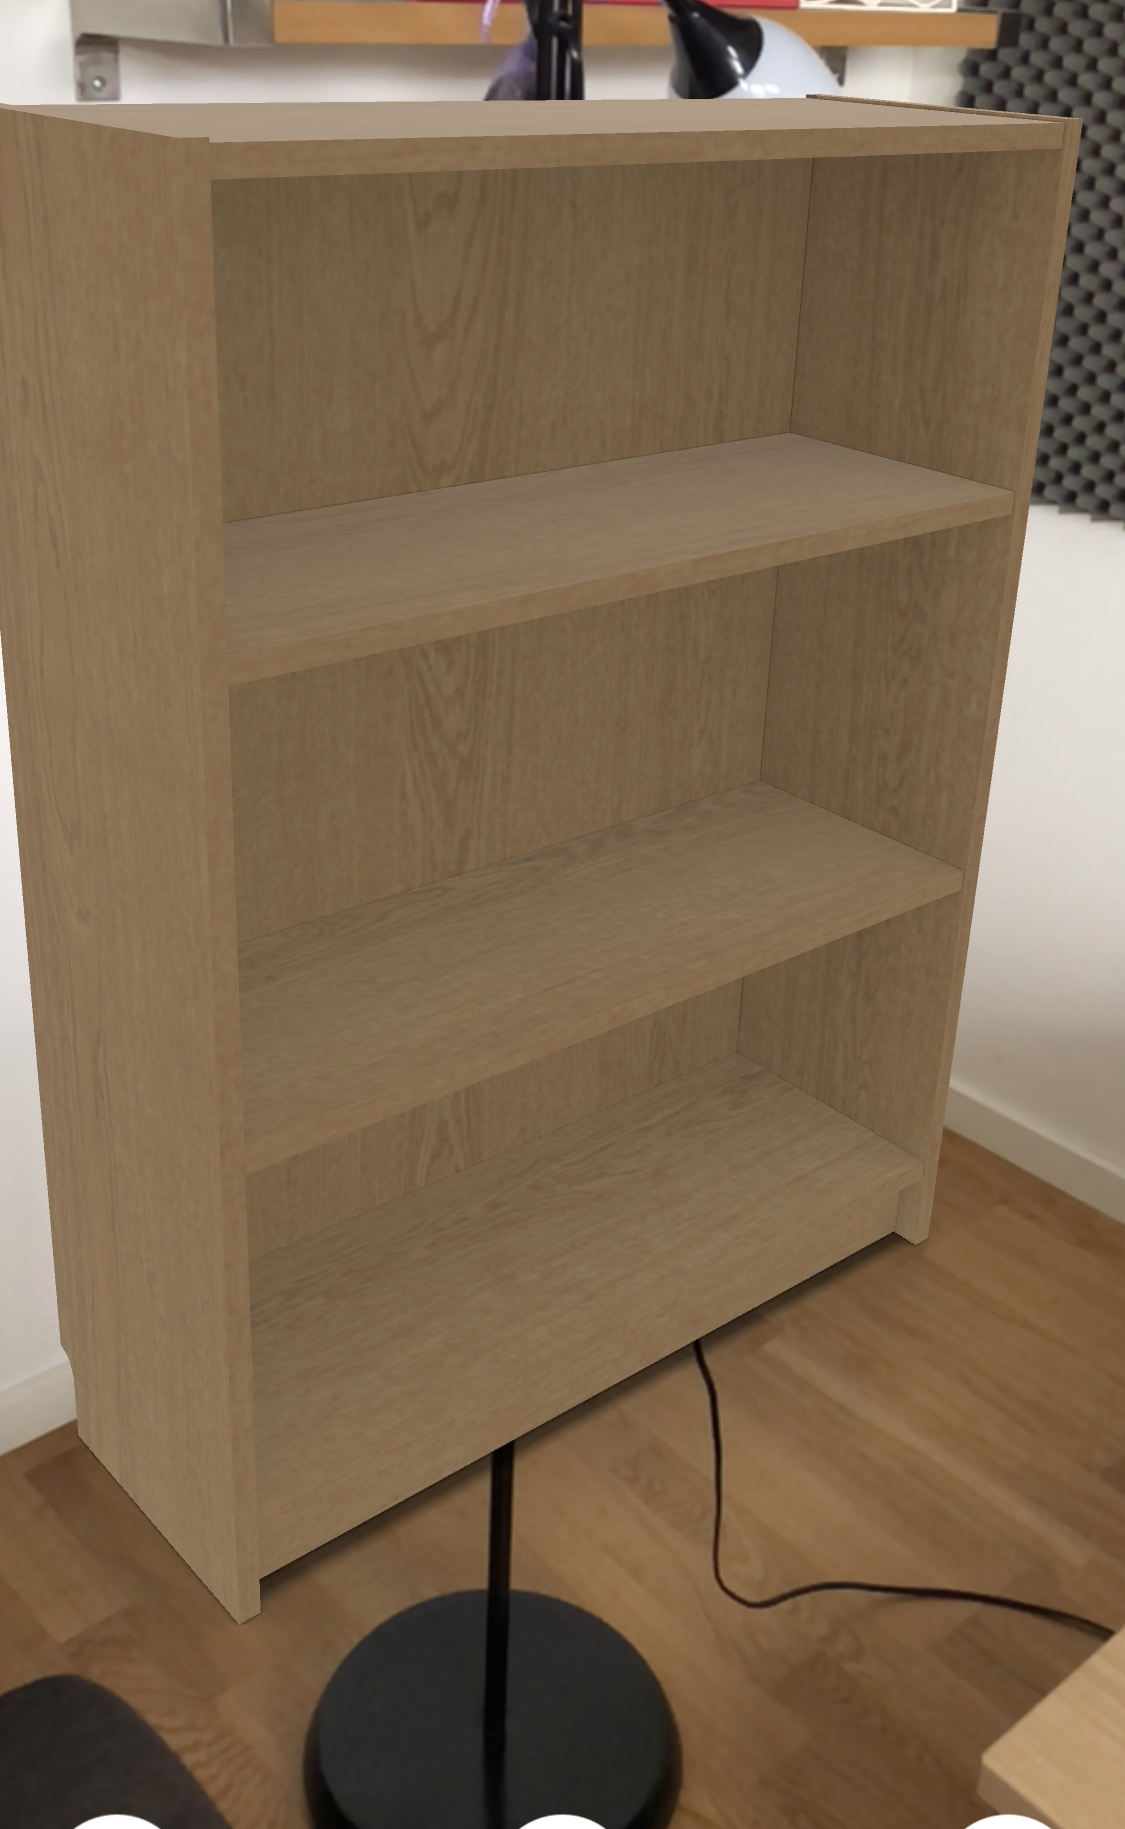
\includegraphics[width = 0.25\textwidth]{./Images/overlapping1.jpg} 
\caption{Book shelf rendered in a corner. To the left no objects in front so it looks realistic.On the right, the book shelf has a lamp in front of it.}
\label{fig:occlusion}
\end{center}
\end{figure}

One of the current problems with Augmented Reality for us is that the models are rendered on top of the real world. When there are no other object in the scene and we just have a simple plane to render one, the result can look decently realistic. However, when other objects are in the scene, the  illusion of realism is easily lost. Example of this can be seen in figure \ref{fig:occlusion}. 

A way to solve this problem would be to create a 3D model of the real world, to be able to find foreground objects and thus, add a transparency mask on the object we wish to render in the real world to increase the effect of illusion that it is actually there.

As of now it is not possible with ARKit to do this in a real time fashion. However, there are scholars working on solutions for the occlusion problem in augmented reality, such as Shah, Niyati \cite{occlusion}.

\newpage
